%%
% The BIThesis Template for Bachelor Graduation Thesis
%
% 北京理工大学毕业设计(论文)第一章节 —— 使用 XeLaTeX 编译
%
% Copyright 2020 Spencer Woo
%
% This work may be distributed and/or modified under the
% conditions of the LaTeX Project Public License, either version 1.3
% of this license or (at your option) any later version.
% The latest version of this license is in
%   http://www.latex-project.org/lppl.txt
% and version 1.3 or later is part of all distributions of LaTeX
% version 2005/12/01 or later.
%
% This work has the LPPL maintenance status `maintained'.
%
% The Current Maintainer of this work is Spencer Woo.
%
% 第一章节

%%==================================================
%% chapter01.tex for BIT Master Thesis
%% modified by yang yating
%% version: 0.1
%% last update: Dec 25th, 2016
%%==================================================
\chapter{无人机编队整体控制逻辑、仿真环境以及硬件选型}
\label{chap:hardware}
本章主要介绍无人机编队的编队控制算法之外的系统组成部分;之后介绍无人机编队的整体的控制的实现逻辑,之后将介绍无人机编队的动力学仿真环境的搭建。
最后将介绍本次设计之中所用到的无人机型号,自动驾驶仪硬件以及姿态自动驾驶仪内环基本控制逻辑。
\section{无人机编队软件整体控制逻辑}
本部分将介绍完整的软件的控制逻辑以及使用的软件环境。
内环姿态驾驶仪使用的是开源自动驾驶仪PX4。PX4是一个为无人机或者其他无人系统设计的高度模块化、可定制化的开源自动驾驶仪软件系统;
PX4软件本身提供了丰富的应用程序接口(API)以及软件开发工具包(SDK),可以与$ROS$等机器人操作系统进行数据交互。下图展示了$PX4$
的软件架构:
\begin{figure}[H]
    \centering
    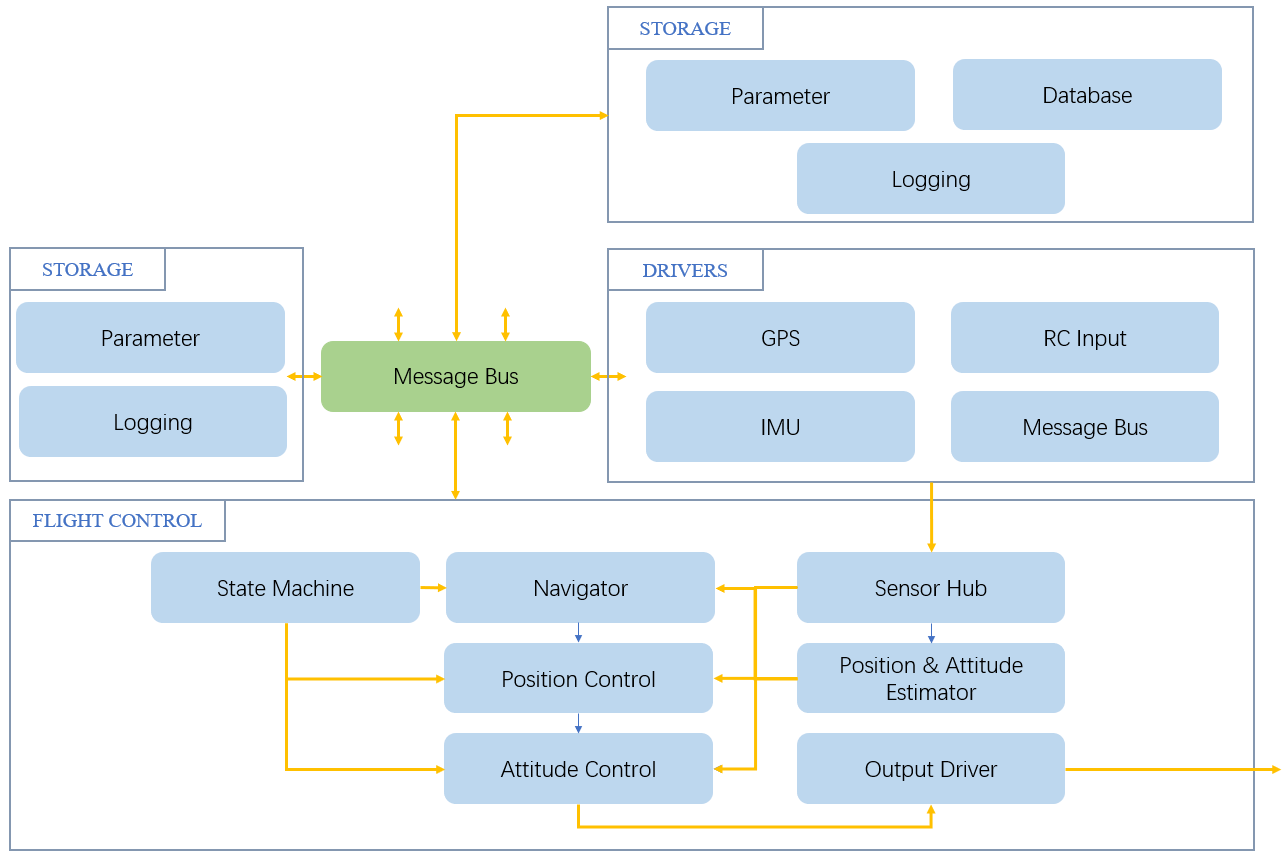
\includegraphics[width=0.8\textwidth]{figures/c4/PX4_archticher.png}
    \caption{PX4软件架构}\label{fig:PX4_archticher.png}
\end{figure}

编队控制算法所运行的软件环境是$ROS$($Robot$ $Operating$ $System$)。$ROS$是一个适用于机器人的开源操作系统。
它提供了操作系统应有的服务,包括硬件抽象,底层设备控制,常用函数实现,进程间消息传递,以及包管理。
它也提供用于获取、编译、编写、和跨计算机运行代码所需的工具和库函数。本次使用的应用程序接口是$ROS$下的$mavros$功能包,
本功能包的作用是:将来自自动驾驶仪的无人机状态数据由$mavlink$通信协议转换为$ROS$的进程间的通讯的协议;
将来自编队控制器的姿态驾驶仪内环的期望姿态角以及期望油门值按照$mavlink$的协议进行编码,从而起到沟通编队控制器以及姿态驾驶仪内环的桥梁作用。
\section{无人机软硬件环境选配}
本文所设计的编队控制器是以开源自动驾驶仪$PX4$的内环为基础的,$PX4$的内环自动驾驶仪运行在$Pixhawk$这一开源硬件之上,成为上层控制的下位机(slave computer):
编队控制算法运行在具有$ROS$环境的上位机(host computer)中;
整体的软件硬件选配关系如下图所示:
\begin{figure}[H]
    \centering
    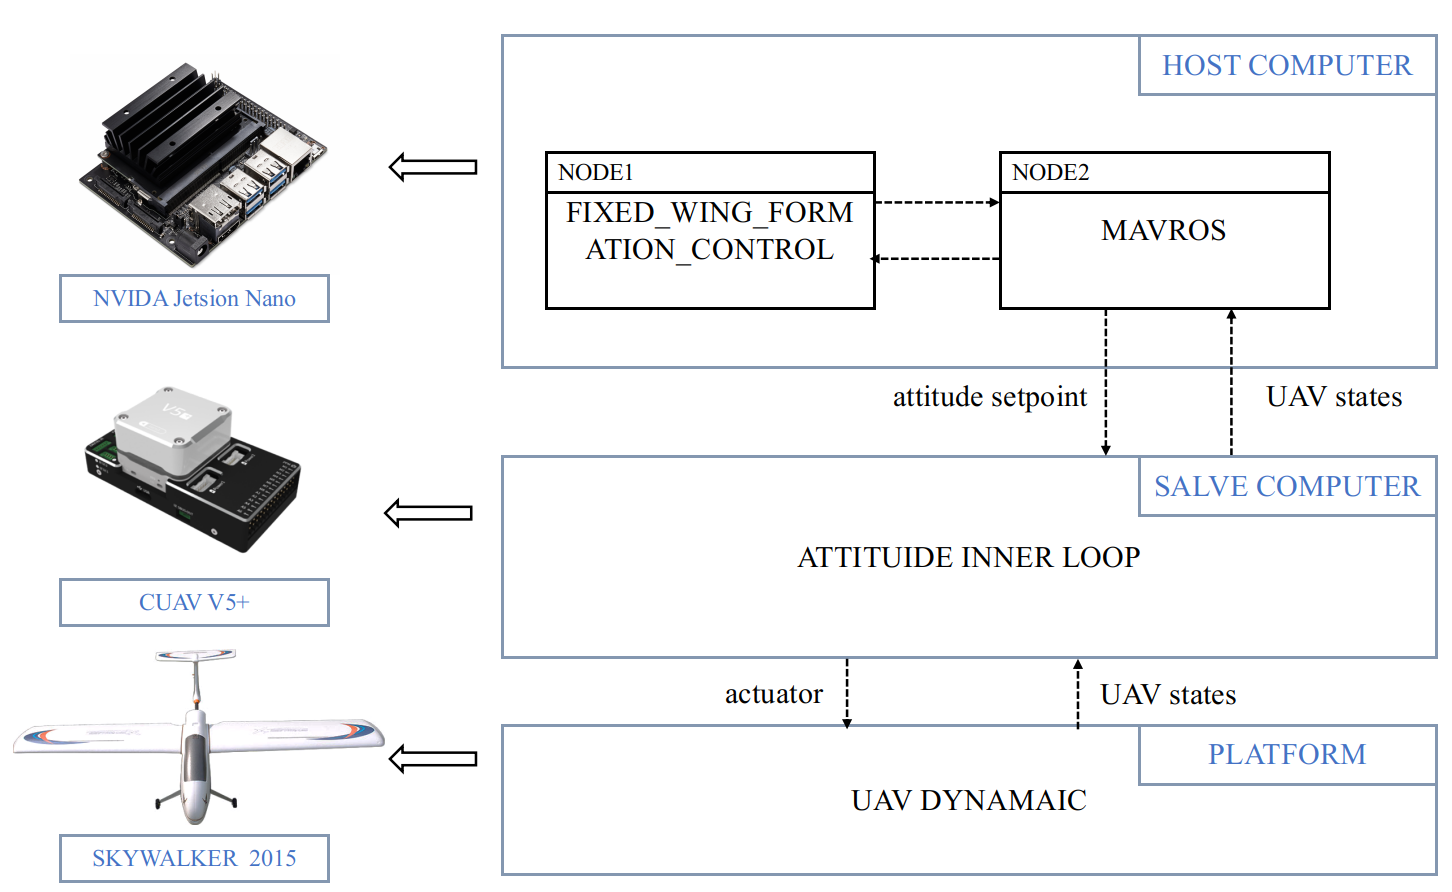
\includegraphics[width=1\textwidth]{figures/c4/c4-soft-hard.png}
    \caption{硬件软件选配关系}\label{fig:c4-soft-hard.png}
\end{figure}
\section{无人机编队动力学仿真环境}
所谓无人机动力学仿真环境,是在考虑无人机的空气动力的作用基础基础之上搭建的仿真环境,相较于控制器的数学仿真,此种仿真环境考
虑了无人机作为一个实际的被控系统而存在的过渡过程,不确定性以及扰动因素,将更加符合无人机飞行时的实际状态。
本次动力学仿真环境基于$Gazebo$这一通用的开源仿真环境仿真环境的。
\begin{figure}[H]
    \centering
    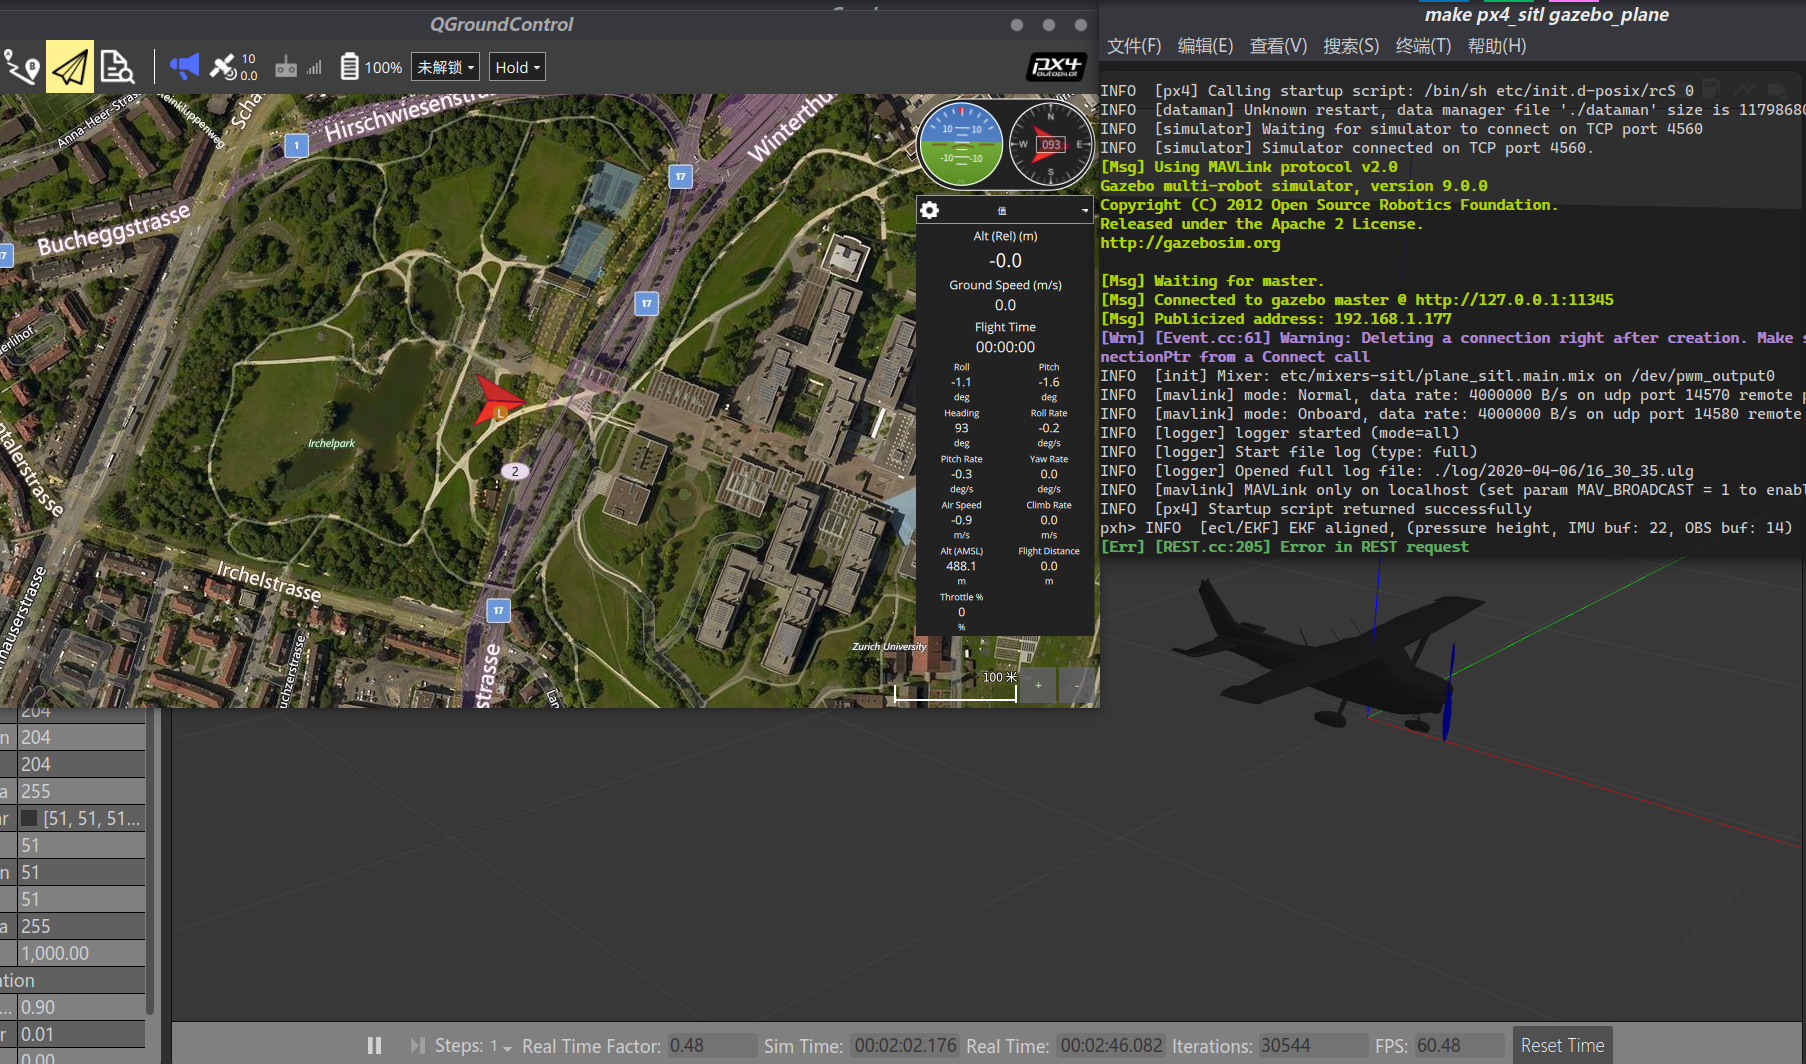
\includegraphics[width=0.75\textwidth]{figures/c4/Gazebo.png}
    \caption{Gazebo仿真环境}\label{fig:c4-Gazebo}
\end{figure}

仿真之中的飞机的动力学模型由Gazebo仿真环境给出,可自定义飞机的质量,推力等参数;仿真之中的传感器数据由Gazebo产生,由PX4读取,作为
真实环境之中的传感器数据的仿真。基于$ROS$的编队控制程序同时运行,通过mavros等程序API进行数据交互,完成动力学仿真。
相应的仿真程序之间的逻辑关系如下图所示:
\begin{figure}[H]
    \centering
    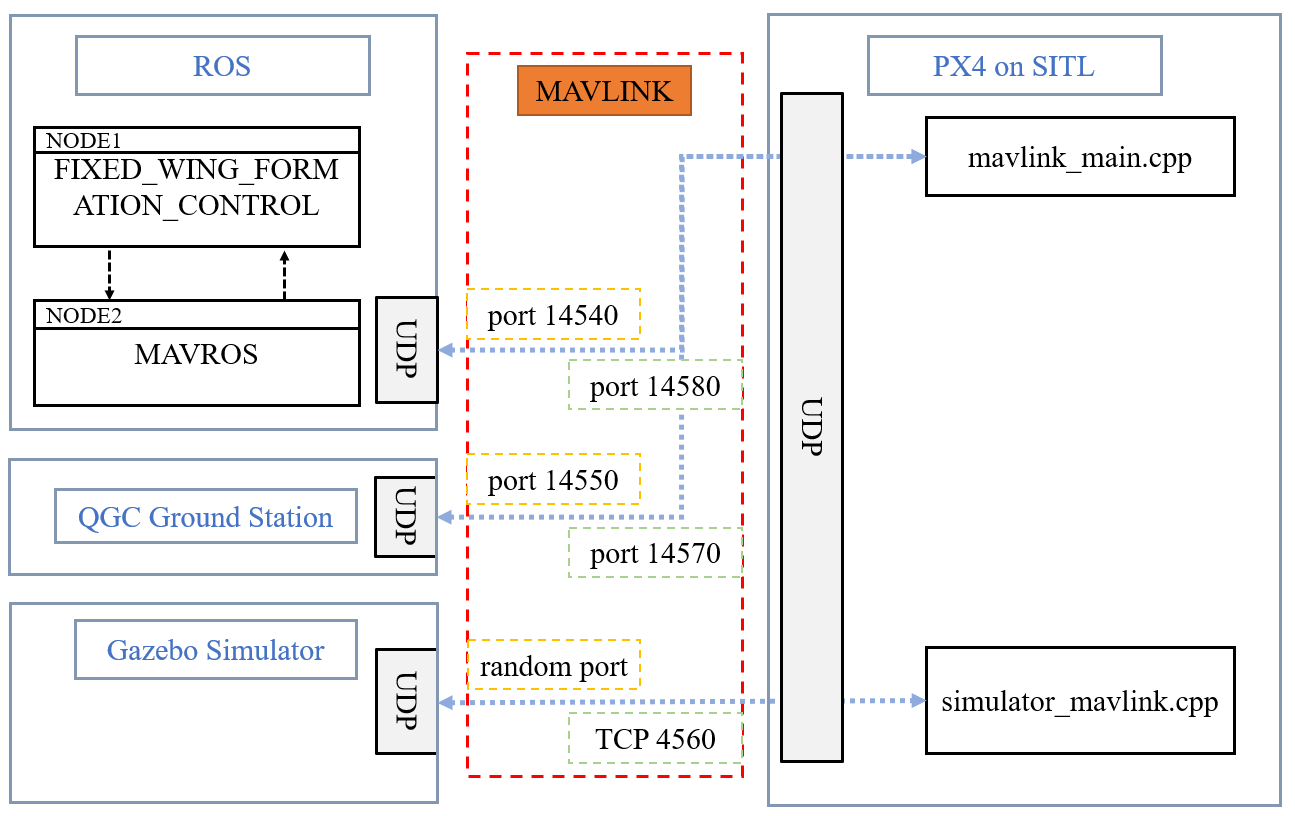
\includegraphics[width=0.75\textwidth]{figures/c4/px4_sitl_overview.png}
    \caption{编队控制仿真逻辑}\label{fig:px4_sitl_overview}
\end{figure}
